\documentclass{article}
\usepackage{fontenc}
\usepackage[ngerman]{babel}
\usepackage[utf8]{inputenc}
\usepackage{graphicx}
\usepackage{grffile}
\usepackage{subcaption}
\usepackage[export]{adjustbox}
\graphicspath{ {../pics/Blatt 2} }
\usepackage{alphalph}
\DeclareUnicodeCharacter{2028}{\linebreak}
\usepackage{hyperref}
\usepackage{listings}
\usepackage{color}

\definecolor{dkgreen}{rgb}{0,0.6,0}
\definecolor{gray}{rgb}{0.5,0.5,0.5}
\definecolor{mauve}{rgb}{0.58,0,0.82}

\lstset{frame=tb,
  language=Java,
  aboveskip=3mm,
  belowskip=3mm,
  showstringspaces=false,
  columns=flexible,
  basicstyle={\small\ttfamily},
  numbers=left,
  numberstyle=\tiny\color{gray},
  keywordstyle=\color{blue},
  commentstyle=\color{dkgreen},
  stringstyle=\color{mauve},
  breaklines=true,
  breakatwhitespace=true,
  tabsize=3
}
\usepackage{datetime}
\newdateformat{myformat}{\THEDAY{ten }\monthname[\THEMONTH], \THEYEAR}

\begin{document}
	\begin{titlepage}
		\centering
		{\scshape\LARGE
			Ereignisdiskrete Systeme
			\par}
		\vspace{1.5cm}
		{\huge\bfseries Praktikum Blatt 2 - Simulink\par}
		\vspace{1.5cm}
		{\LARGE\itshape Jan Kristel, Alexandra Moritz\par}
		\vfill
			Aufsicht von Frau Rembold\par
			
		\vfill	
			{\large \today \par}	
		
	\end{titlepage}
	
	\tableofcontents
	\newpage
	
	\section{Grundlagen}
		\subsection{Welcher Übertragungstyp?}
			\renewcommand{\thesubsubsection}{\alph{subsubsection})}
			\subsubsection{}
				$$h_1(t) = \frac{\frac{1}{4}}{s}$$
				Es handelt sich um die Sprungfunktion eines I-Glied
			\subsubsection{}
				$$h_2(t) = \frac{s}{s + 1}$$
				Die Sprungfunktion ist von einem $DT_1$-Glied.
			\subsubsection{}
				$$h_3(t) = \frac{2}{0,95s^2 + 0,19s +1}$$
				Das Bild zeigt die Sprungfunktion eines $PT_2$-Glieds an.
			\subsubsection{}
				$$h_4(t) = \frac{1}{s + 1}$$
				Hierbei sieht man den Graphen der Sprungfunktion eines verzögerten $PT_1$-Glieds.
		\subsection{Relevante Parameter}
			\subsubsection{}
				\begin{itemize}
					\item $K_I = \frac{1}{4} \rightarrow$ dient der Steigung. Dies lässt sich aus dem Bild/Graph ablesen.
				\end{itemize}
			\subsubsection{}
				\begin{itemize}
					\item $K_D = \frac{1}{1} = 1$. Dies sorgt für ein bestehendes $s$ im Zähler.
					\item $T_1 = 1$, was für ein vorhandenes $s$ im Nenner sorgt.
				\end{itemize}
			\subsubsection{}
				\begin{itemize}
					\item $K_P = 2$, durch ablesen bestimmt.
					\item $T_2$ und $T_1$ müssen berechnet werden:
						\begin{itemize}
							\item $$\vartheta  = ln\Big(\frac{\Delta_1}{\Delta_2} \Big) = ln \Big(\frac{1,5}{1}\Big) = 0,3$$ $\rightarrow \Delta_1 und \Delta_2$ sind die ersten beiden Schwingungen der Sprungfunktion, nachdem diese den $K_P = 2$ gekreuzt haben.
							\item $$d = \frac{\vartheta}{\sqrt{\pi^2 + \vartheta^2}} = \frac{0,3}{\sqrt{\pi^2 + ^2}} = 0,098$$
							\item $$\omega_e = \frac{2\cdot \pi}{T_e} = \frac{2\cdot \pi}{6} = 1,047$$ $\rightarrow T_e$ lässt sich aus dem Graphen abschätzen. Das ist die Dauer für die ersten vollständige Schwingung nachdem $K_P$ erreicht wurde.
							\item $$\omega_0 = \frac{\omega_e}{\sqrt{1 - d^2}} = \frac{1,047}{\sqrt{1 - 0,098^2}} = 1,052$$ 
							\item $$T_2 = \frac{1}{\omega_0} = \frac{1}{1,052} = 0,95$$
							\item $$T_1 = 2\cdot d \cdot T_2 = 2 \cdot 0,098 \cdot 0,95 = 0,19$$
						\end{itemize}
				\end{itemize}
			\subsubsection{}
				\begin{itemize}
					\item $K_P = \frac{1}{1} = 1$ Dies lässt sich wieder aus dem Graph ablesen.
					\item $T_1 = 1$
					\item $t = 1 \rightarrow$ die Verzögerung $t$ lässt sich ablesen und in Simulink durch ein extra Verzögerungsglied einstellen.
				\end{itemize}
\newpage
		\subsection{Überprüfung durch Simulink}
			\subsubsection{}
				\begin{figure}[h]
					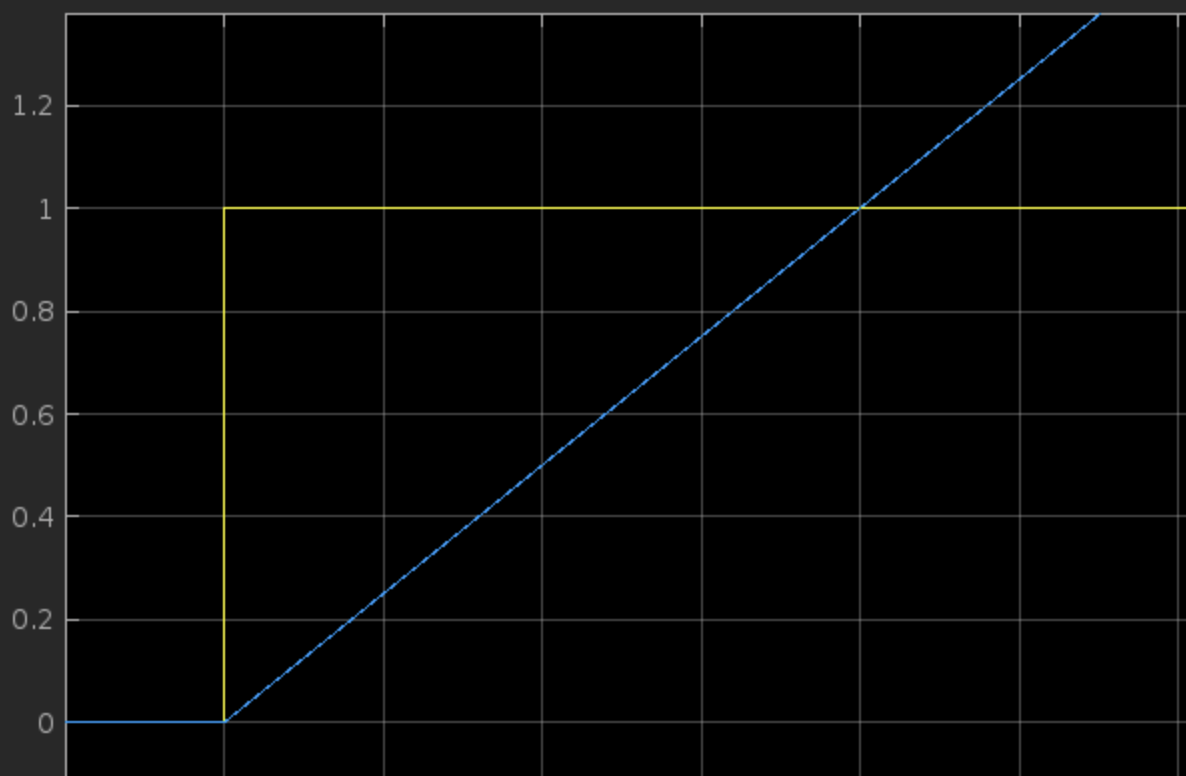
\includegraphics[scale=0.22, center]{./Sprungfunktion_I_Glied.png}
					\caption{Graph einer Sprungfunktion eines I-Glieds.}
					\label{fig1: Springfunktion-I-Glied}
				\end{figure}	
			\subsubsection{}
				\begin{figure}[h]
					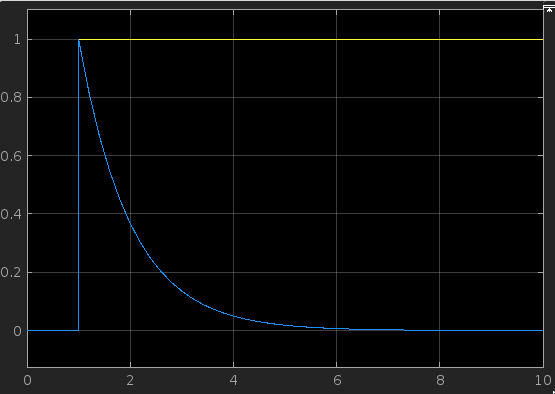
\includegraphics[scale=0.47, center]{./Sprungfunktion_DT_1_Glied.png}
					\caption{Graph einer Sprungfunktion eines $DT_1$-Glieds.}
					\label{fig2: Springfunktion-DT-1-Glied}
				\end{figure}	
\newpage
			\subsubsection{}
				\begin{figure}[ht]
					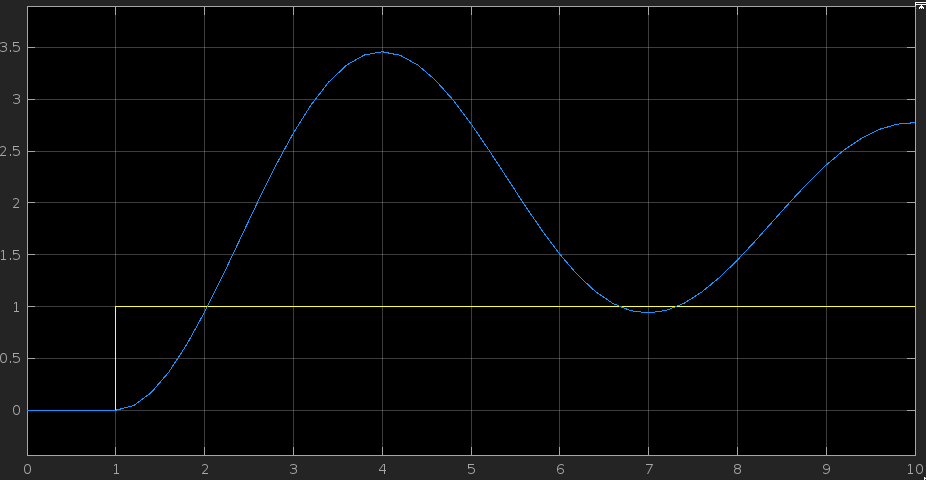
\includegraphics[scale=0.4, center]{./Sprungfunktion_PT_2_Glied.png}
					\caption{Graph einer Sprungfunktion eines $PT_2$-Glieds.}
					\label{fig3: Springfunktion-PT-2-Glied}
				\end{figure}	
			\subsubsection{}
				\begin{figure}[ht]
					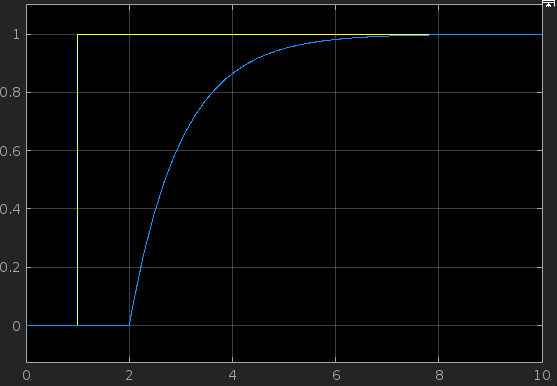
\includegraphics[scale=0.4, center]{./Sprungfunktion_PT_1_Glied_verzoegert.png}
					\caption{Graph einer Sprungfunktion eines um 1 Zeiteinheit verzögertes $PT_1$-Glieds.}
					\label{fig1: Springfunktion-PT-1-Glied}
				\end{figure}	
\newpage
	\section{Optimierung eines einfachen Regelkreises}
	
\end{document}